\section{Results}

\subsection{Validation of the controls}

When conducting \acrlong{de} analysis, the user has to ensure that controls are separated from the the tumours.
Homogeneity among the controls, similarity between the control and tumour counts distribution are also factors that can improve the results.
Despite that the controls should be separated from the tumours, it has been observed for different types of cancer in \acrshort{tcga} that the gene expression follows a similar distribution between the two conditions \cite*{Decamps2021}.

\begin{figure}
    \begin{center}
        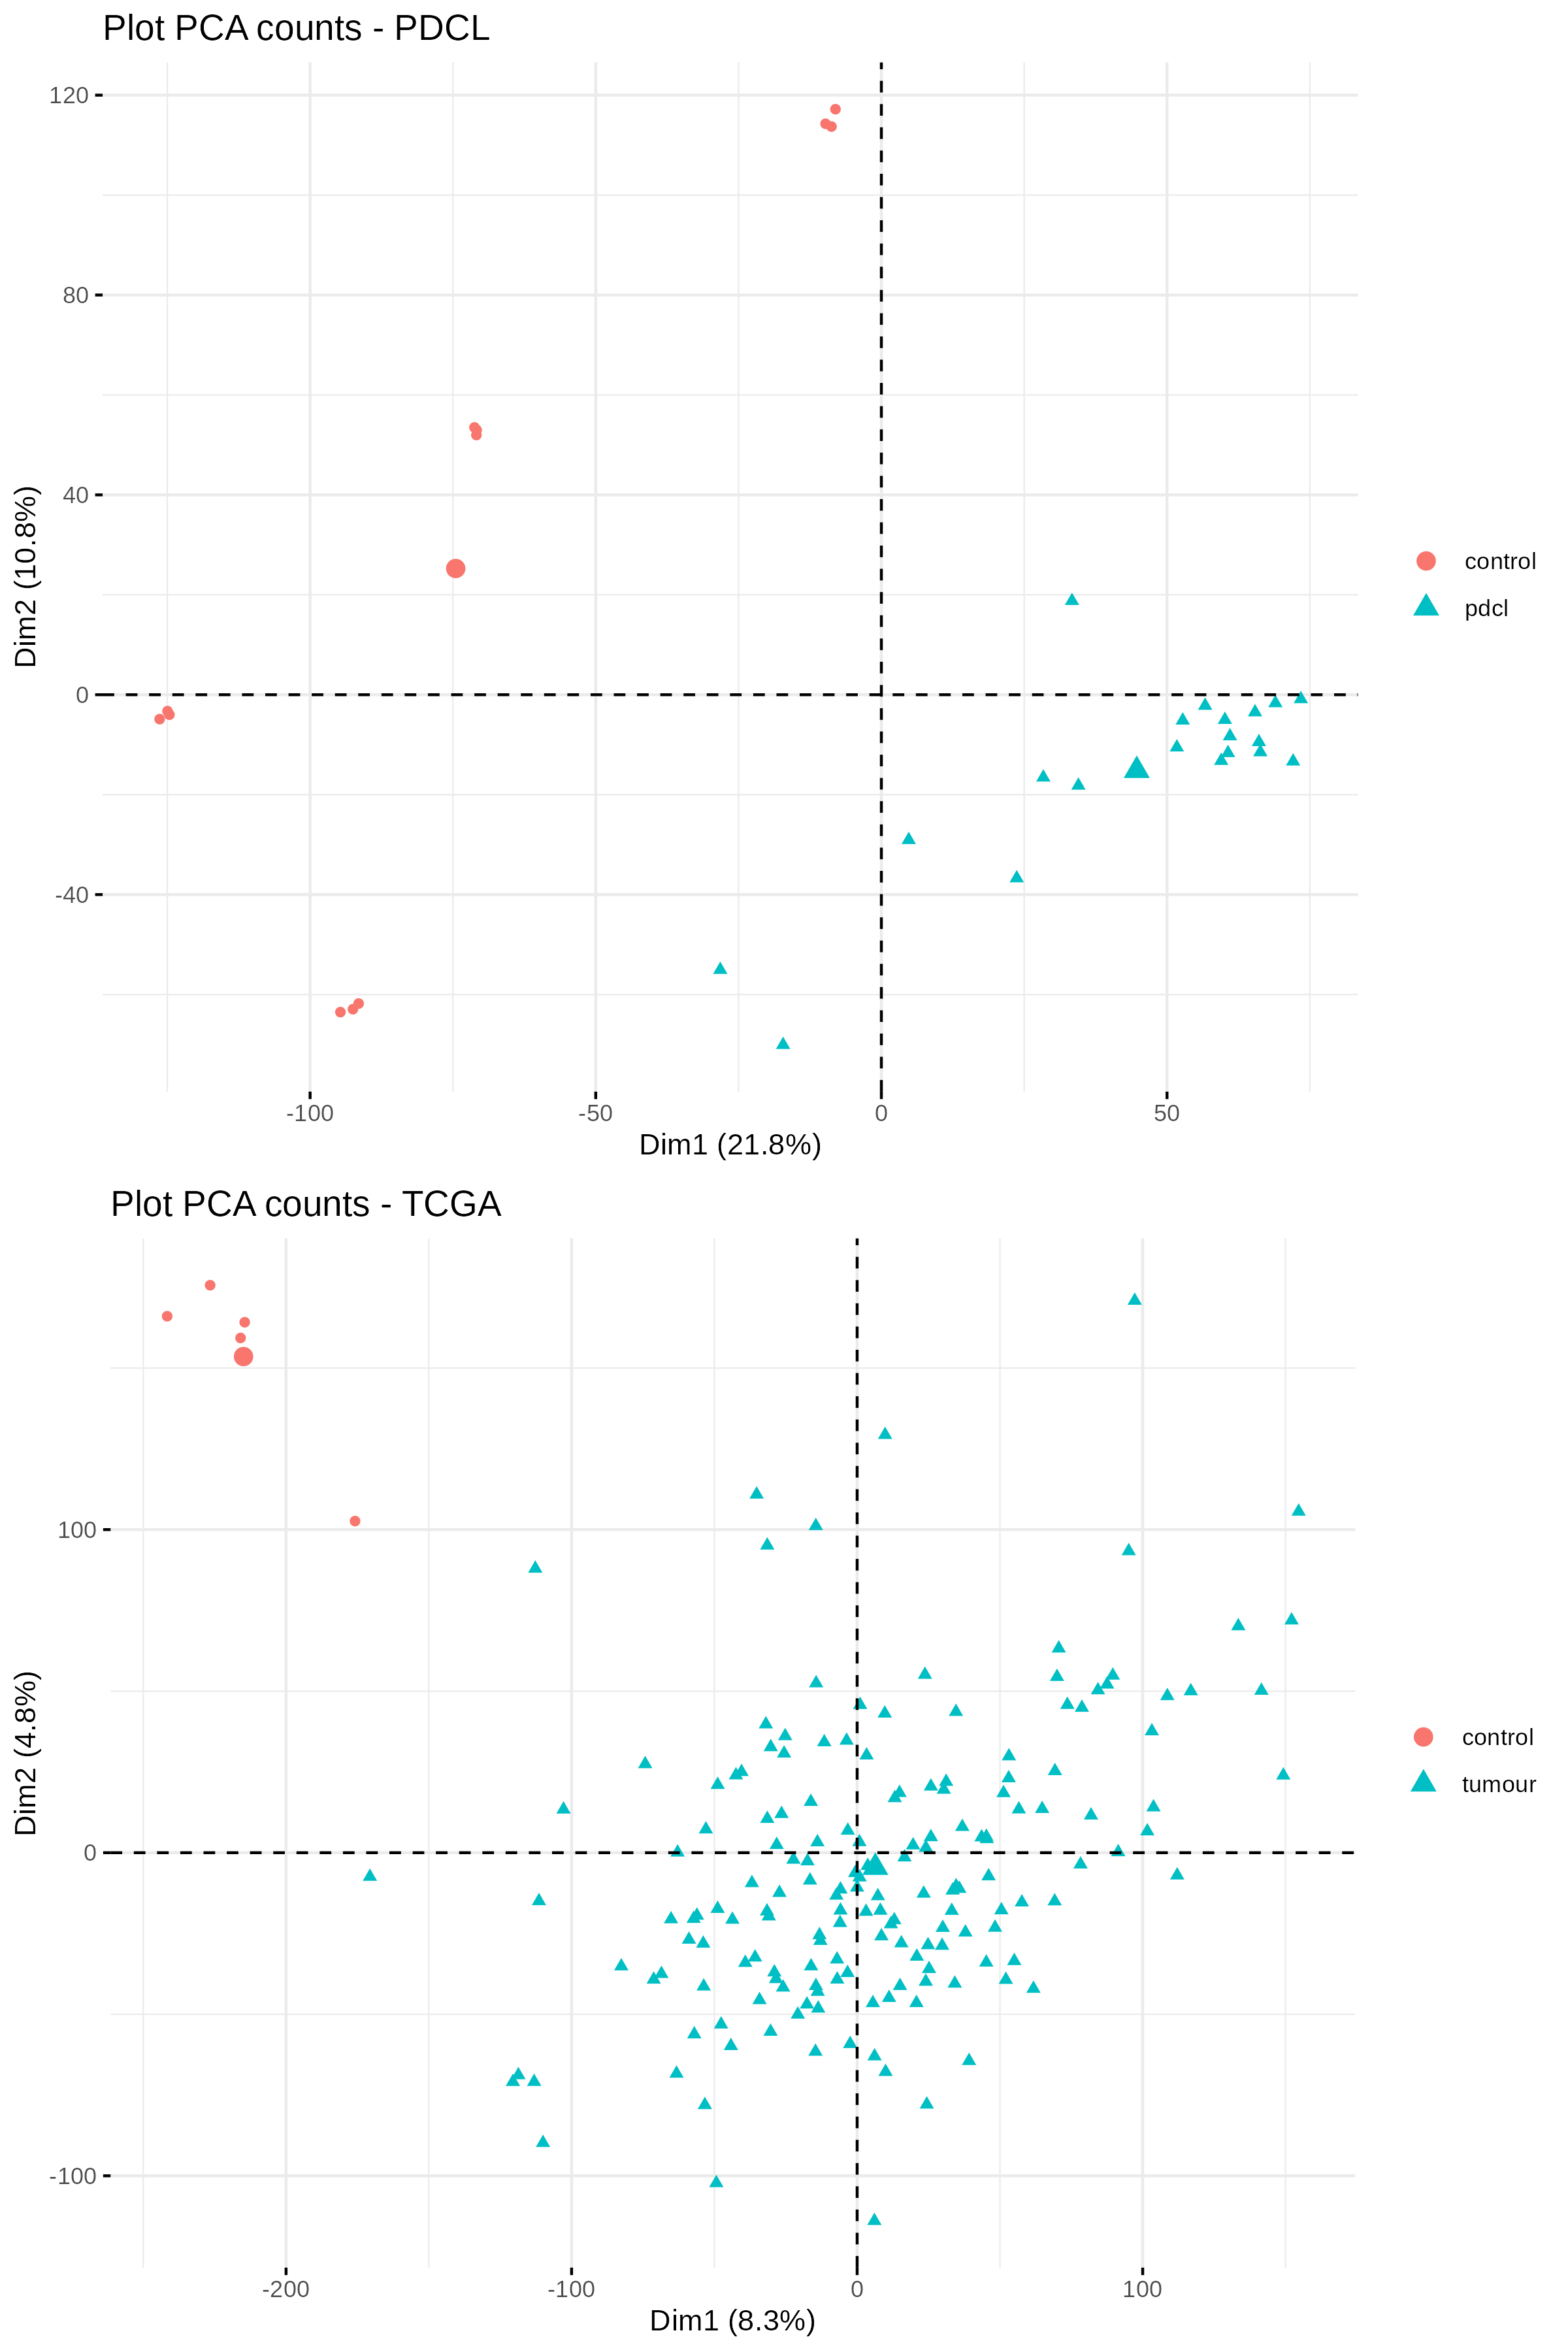
\includegraphics[height=0.8\textheight]{img/pca_plot}
        \caption{
            Plot of the \acrshort{pca} on the counts of control and glioblastoma samples of the \acrshort{pdcl} and \acrshort{tcga} datasets.
            Counts were normalized using the pseudo-log method of the DESeq2 package ( $log_2(count+1)$ ).
        }
        \label{fig:pca-plot}
    \end{center}
\end{figure}

Figure \ref*{fig:pca-plot} shows the results of a \acrfull{pca} performed on the counts normalized using the pseudo-log method from the DESeq2 package ( $log_2(count+1)$ ).
It can be seen that the controls are separated from the tumours  in both the \acrshort{pdcl} and the \acrshort{tcga} datasets by the first two components of the \acrshort{pca}.
The first component explain more variances in the data in the \acrshort{pdcl} datasets with 21\% compared to 8\% with \acrshort{tcga}.
In the \acrshort{tcga} datasets, the tumours samples tend to spread more accross the second component than the controls which seems to pack together while in the \acrshort{pdcl} dataset, controls are more scattered. 

\begin{figure}
    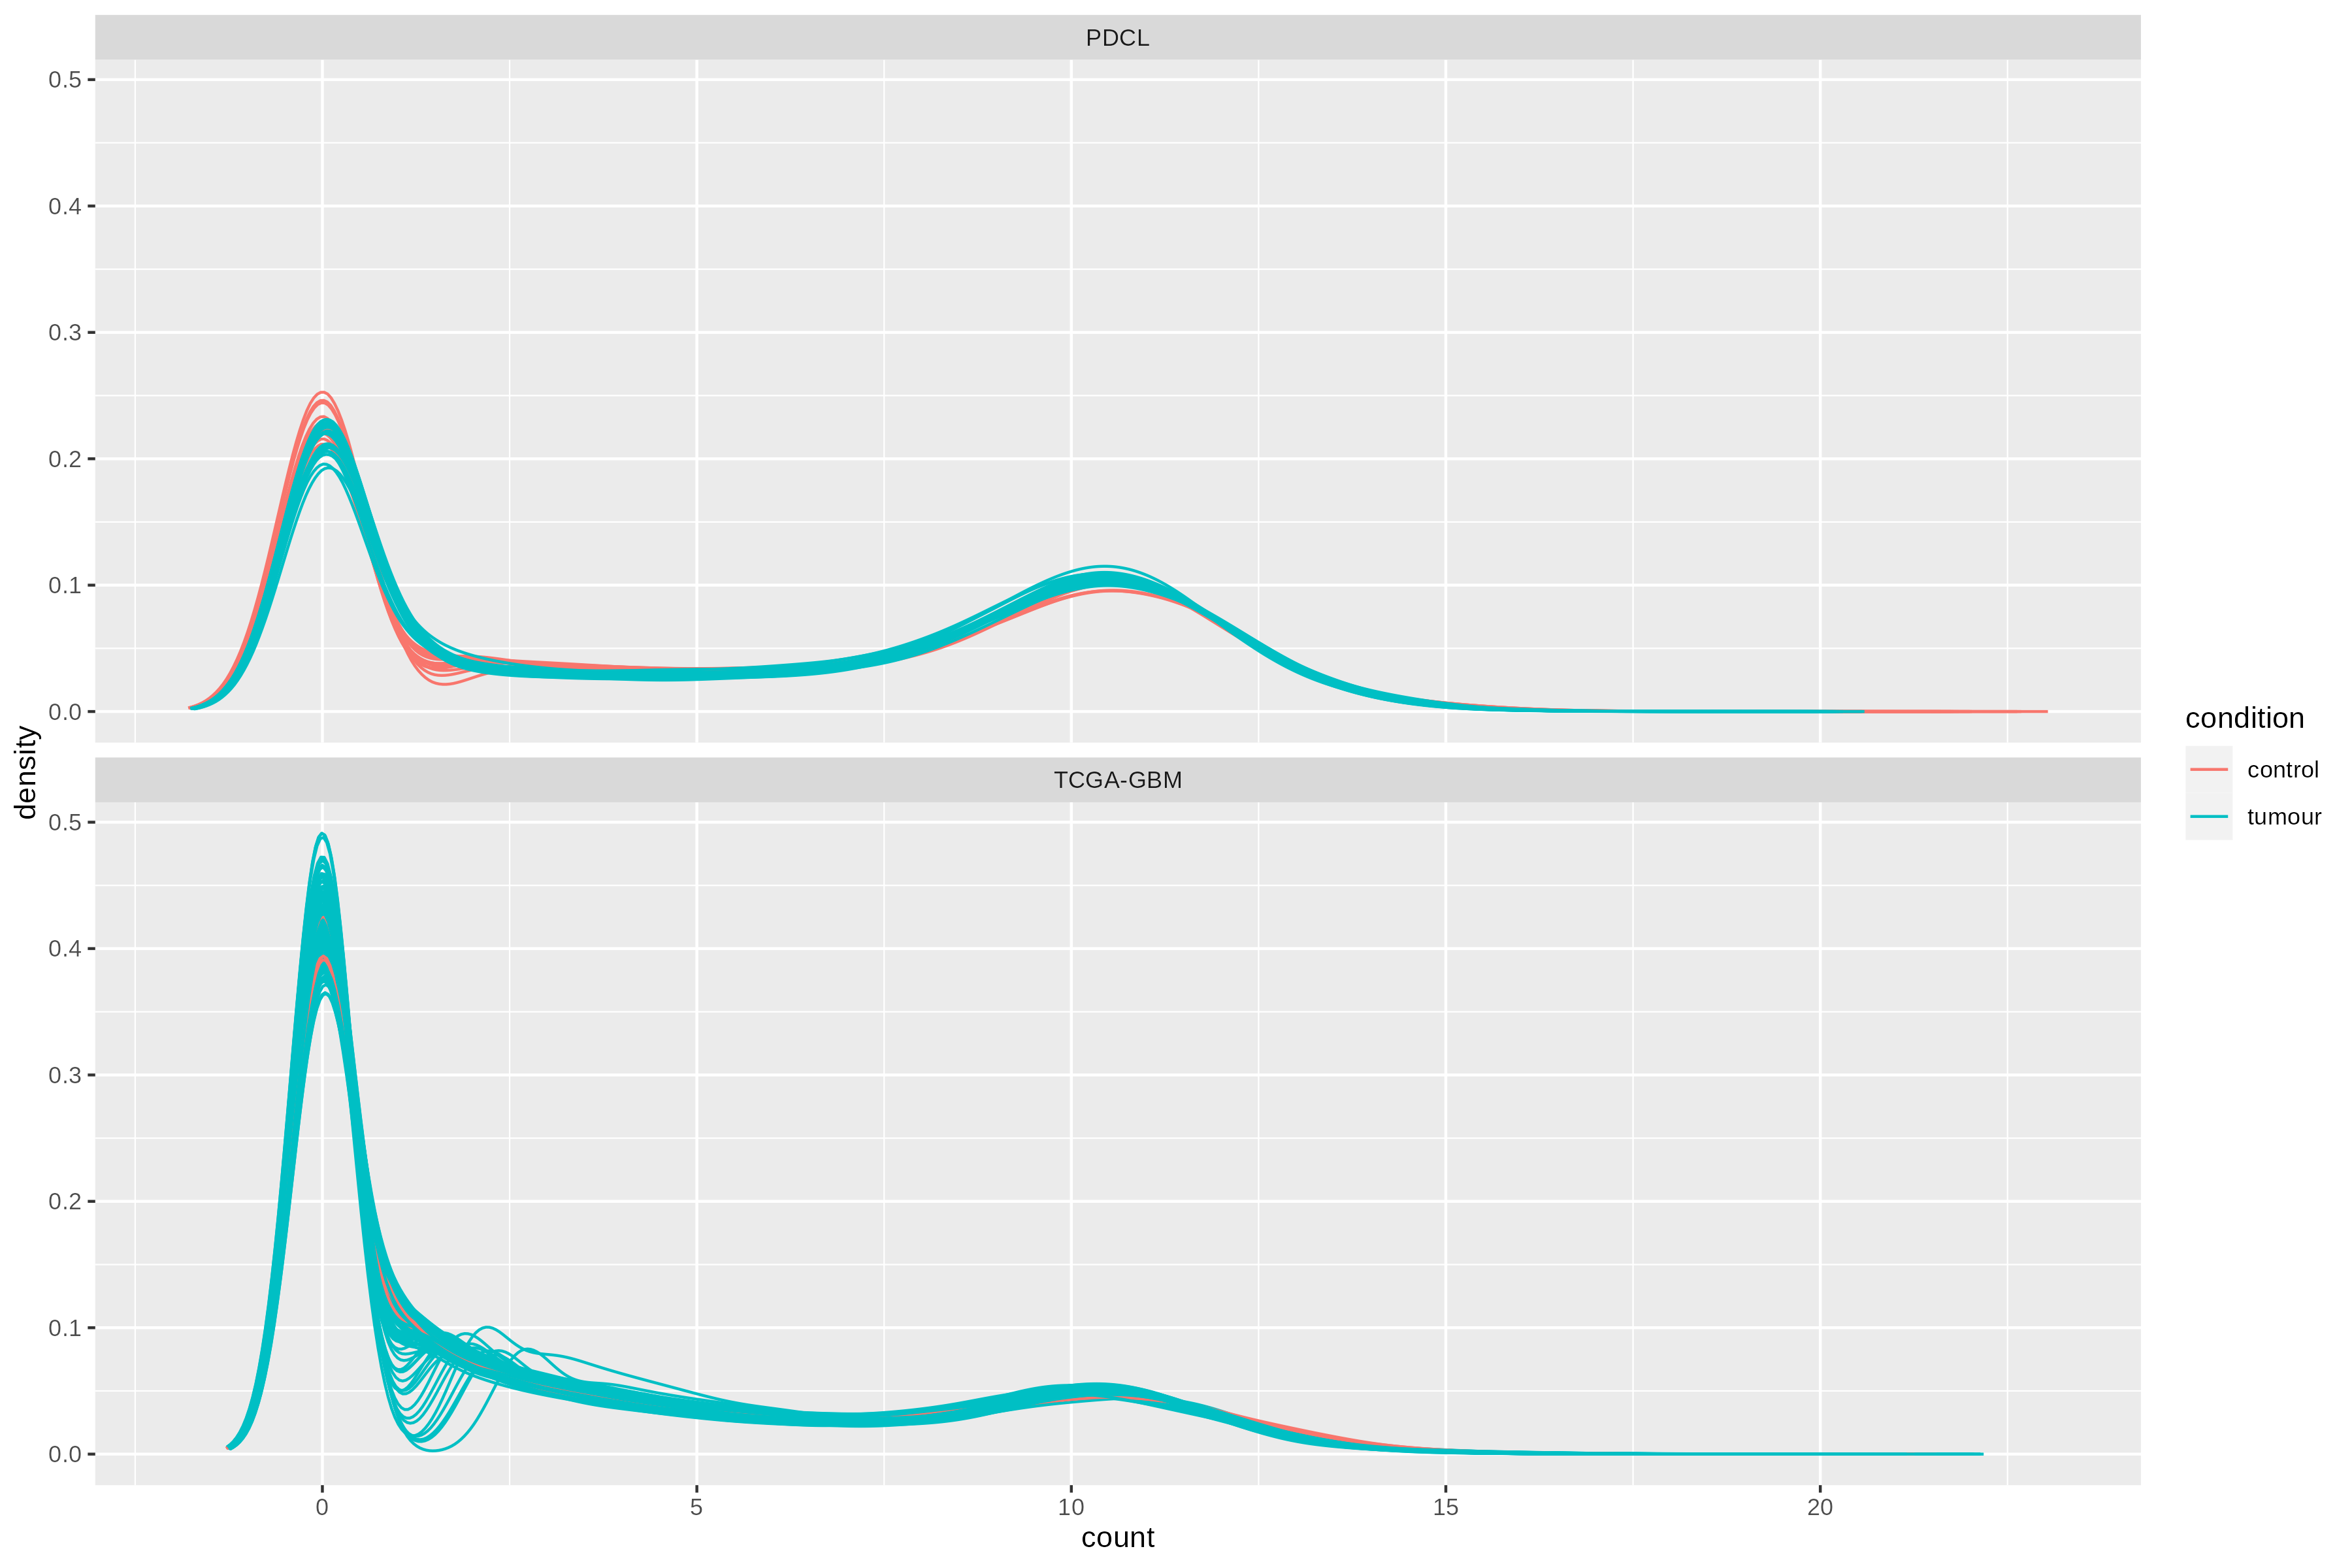
\includegraphics[width=\textwidth]{img/density_plot}
    \caption{
        Plot of the density of the counts in control and glioblastoma samples of the \acrshort{pdcl} and \acrshort{tcga} datasets.
        Counts were normalized using the pseudo-log method of the DESeq2 package ( $log_2(count+1)$ ).
        Each lines represent a different sample.
    }
    \label{fig:density-plot}
\end{figure}

Figure \ref*{fig:density-plot} shows the distribution of normalized gene counts in controls and tumours among both datasets.
Distribution of counts is similar among controls and tumours in both datasets with a similar intensity on the peak between controls and tumours with respect to the dataset.

Together, these data seems to indicate that the controls choosen are suitable to perform the \acrlong{de} analysis then pathway enrichment.

\subsection{Analysis of the deregulated pathways at the population scale}

\subsubsection{Target pathways shows quality of enrichment among the results}

The \acrshort{kegg} database document the processes affected in the case of many diseases including glioma.
During pathway enrichment analysis, one can take one or several target pathways to assess the quality of the results.
For example, Zyla \textit{et al} used the adjusted p-value of the \textit{Glioma} entry (path:hsa05214) as a target pathway to assess the sensitivity of different ranking metrics when studying microarray data from brain tissue \cite*{Zyla2017}.
Here, as we are comparing RNA-Seq data from glioblastoma samples to normal controls, we should expect the adjusted p-value (\acrshort{fdr} in this study) to be below our definied threshold.
The \acrshort{fdr} value for \textit{Glioma} is 0.053 in G:Profiler and 0.83 in \acrshort{gsea} for the \acrshort{pdcl} dataset.
With \acrshort{tcga} data, the \acrshort{fdr} value for \textit{Glioma} is 0.0009 in G:Profiler and 0.005 in \acrshort{gsea}.
It suggests that \acrshort{tcga} data have a better quality than the \acrshort{pdcl} ones.
Controls for the \acrshort{pdcl} dataset are taken from another study \cite*{Lundin2018}, introducing experimental and biological variability independent from disease deregulation.
This can be seen on figure \ref*{fig:pca-plot}, as the controls are more spread in \acrshort{pdcl} than in \acrshort{tcga}.
Controls in the \acrshort{tcga} dataset come from matching samples taken off the original tissue following the exact same protocol as the tumour samples to reduce such variability.
Futhermore, some replicates in the controls of the \acrshort{pdcl} datasets comes from astrocytomas cell lines.
Therefore they are not completely suitable for \acrlong{de} analysis.
It shows that a good set of controls can influence the quality of the results given.

\subsubsection{Differences in deregulated categories among the databases and the tools}

\begin{figure}
    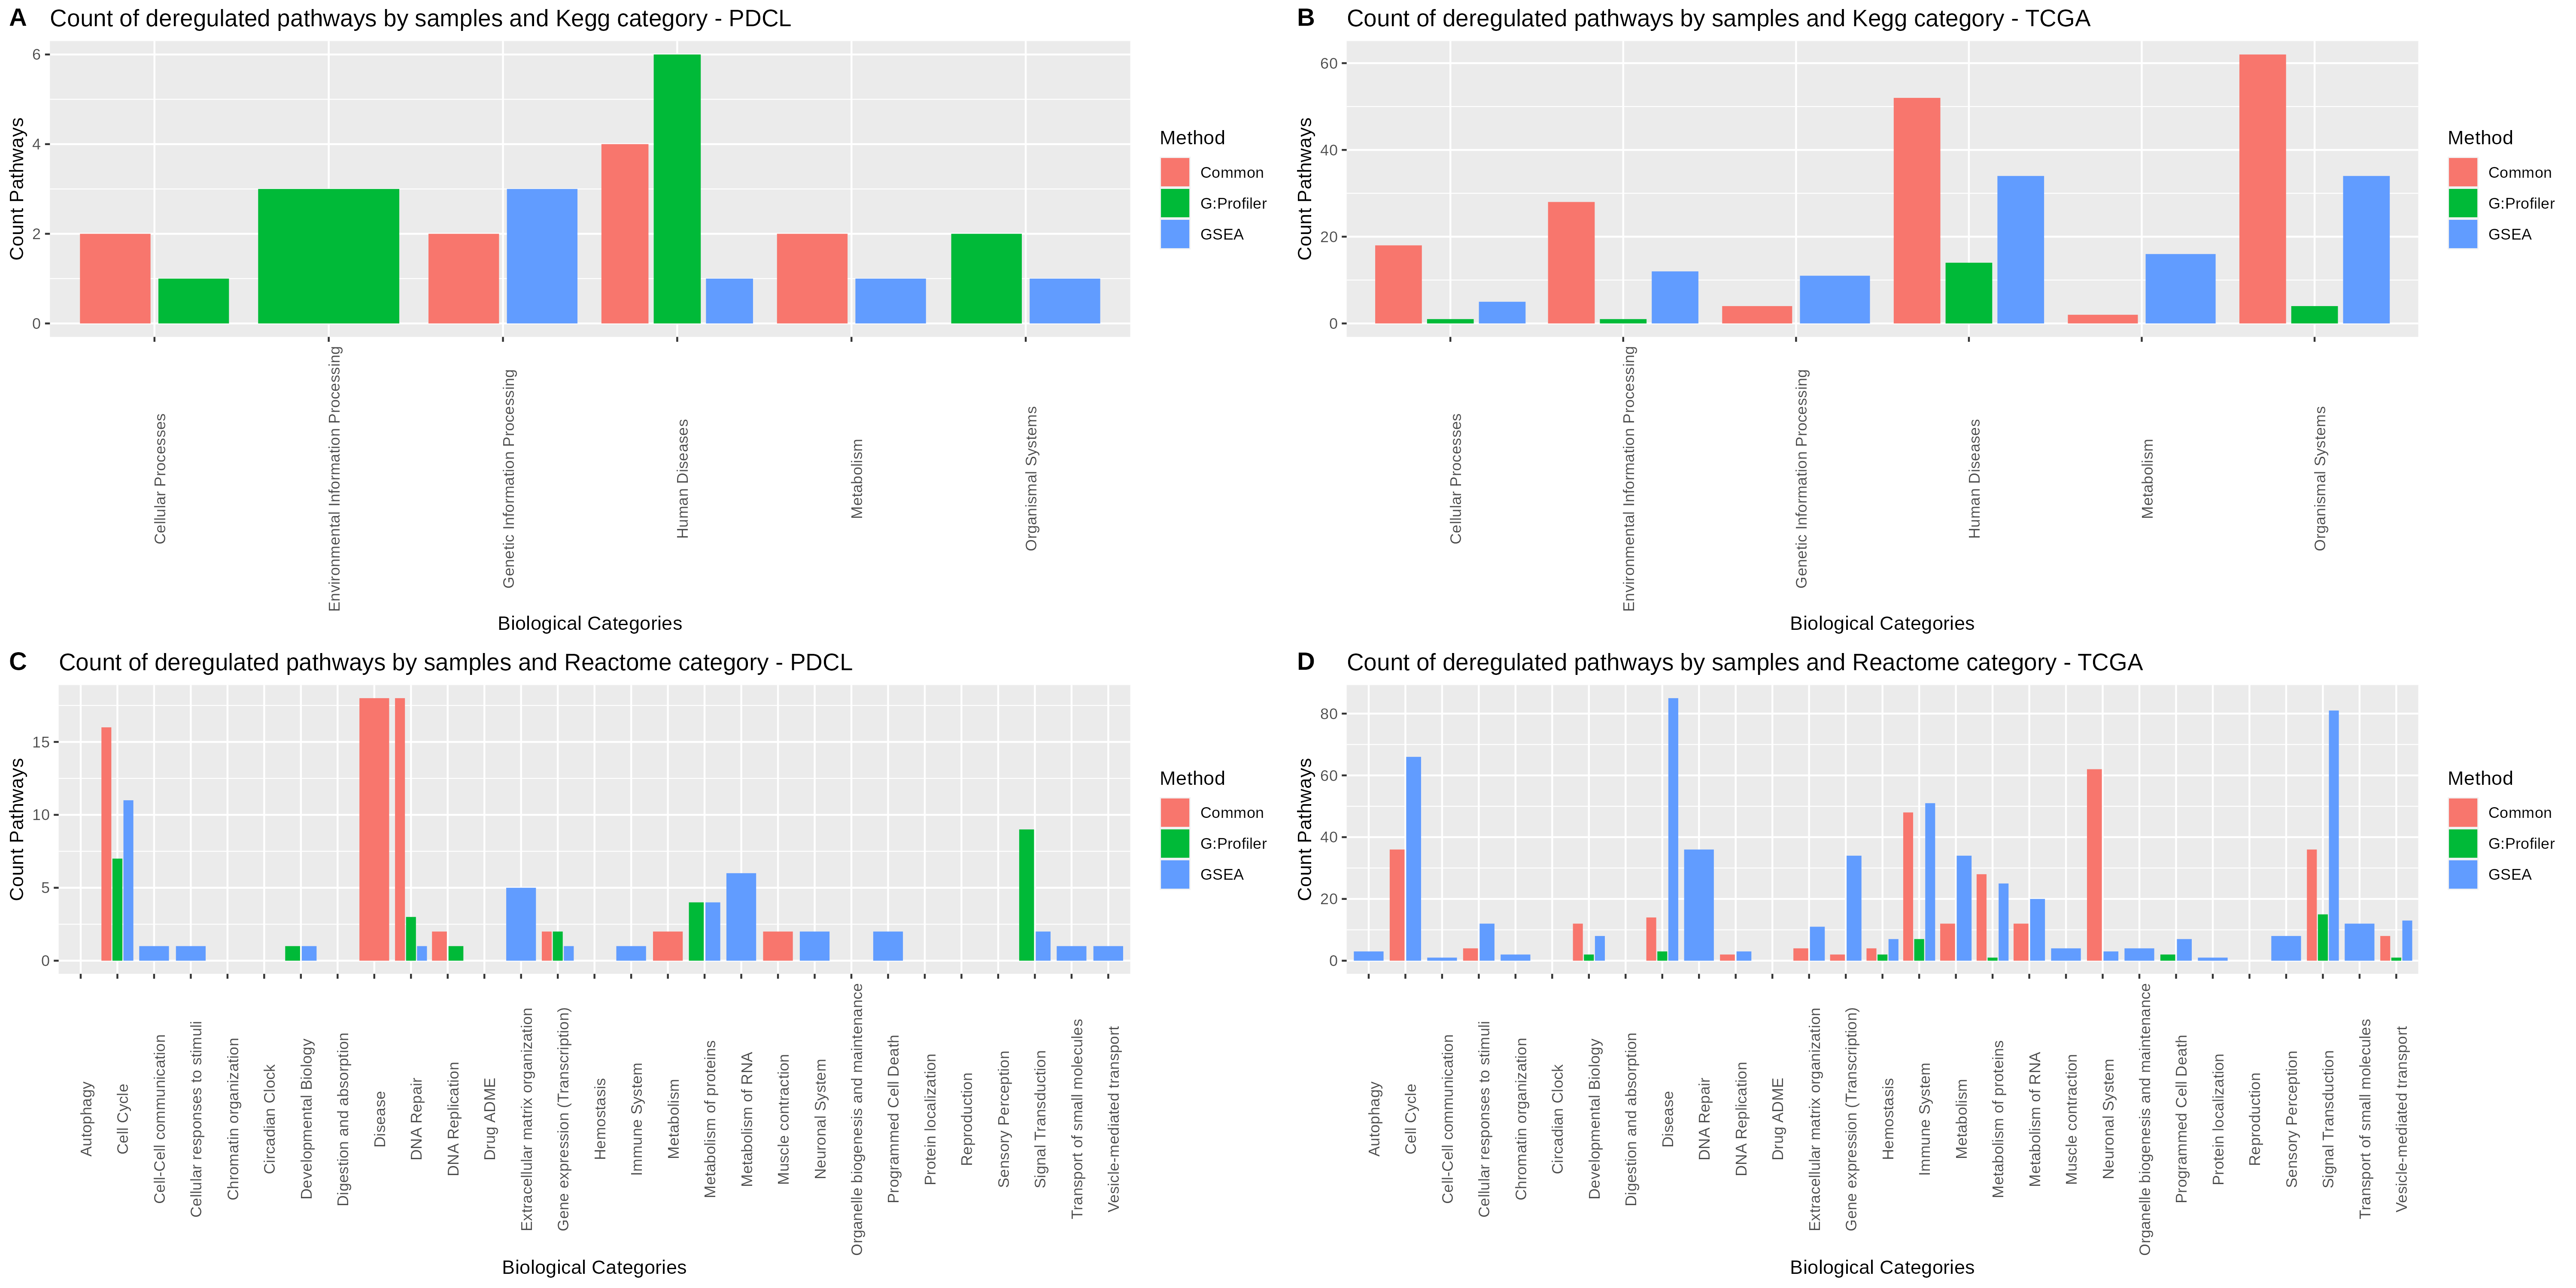
\includegraphics[width=\textwidth]{img/barplot-categ-global}
    \caption{
        Barplot of the count of significantly deregulated pathways for (A) \acrshort{kegg} categories in \acrshort{pdcl}; (B) \acrshort{kegg} categories in \acrshort{tcga}; (C) Reactome categories in \acrshort{pdcl}; (D) Reactome categories in \acrshort{tcga}.
        Pathways are colored wether they are specific to G:Profiler or \acrshort{gsea}, they are significantly enriched in one of the tools, or common, they are significantly enriched in both tools.
    }
    \label{fig:barplot-categ-global}
\end{figure}

As can be seen in figure \ref*{fig:barplot-categ-global}, G:Profiler and \acrshort{gsea} yield different results which are also influenced by the database choosen.
We recommand investigating more than one database when performing pathway enrichment as the choice of the databse may impact the results \cite*{Mubeen2019}.
Most of the time, more pathways are significantly enriched in \acrshort{gsea} compared to G:Profiler.
In some cases, there is no correlation betwen G:Profiler and \acrshort{gsea} results.
For example, the \textit{Organismal Systems} \acrshort{kegg} category is only enriched with pathways specific to G:Profiler or to \acrshort{gsea} with \acrshort{pdcl} data.
Still with the same dataset and database, the \textit{Environmental information Processing} category is only found enriched with G:profiler.
Inversely, the \textit{Disease} Reactome category is enriched with only pathways found using both for the same data.
In addition, Reactome categories like \textit{Circadian Clock} or \textit{Reproduction} are not found enriched in any of the datasets nor tools.
In this study, pathways in the \acrshort{gmt} are filtered only on their size.
Yet, it may be benificial to remove pathways which are not involved in the biological condition being investigated.
The \acrshort{fdr} multiple hypothesis correction method is influenced by the number of null-hypothesis tested, here the number of genes tested for differential expression or pathway tested for enrichment.
Therefore, the more pathways are being tested, the stronger the correction aplied on the p-value is.

\subsubsection{Investigation of selected pathways}

\begin{figure}
    \begin{center}
        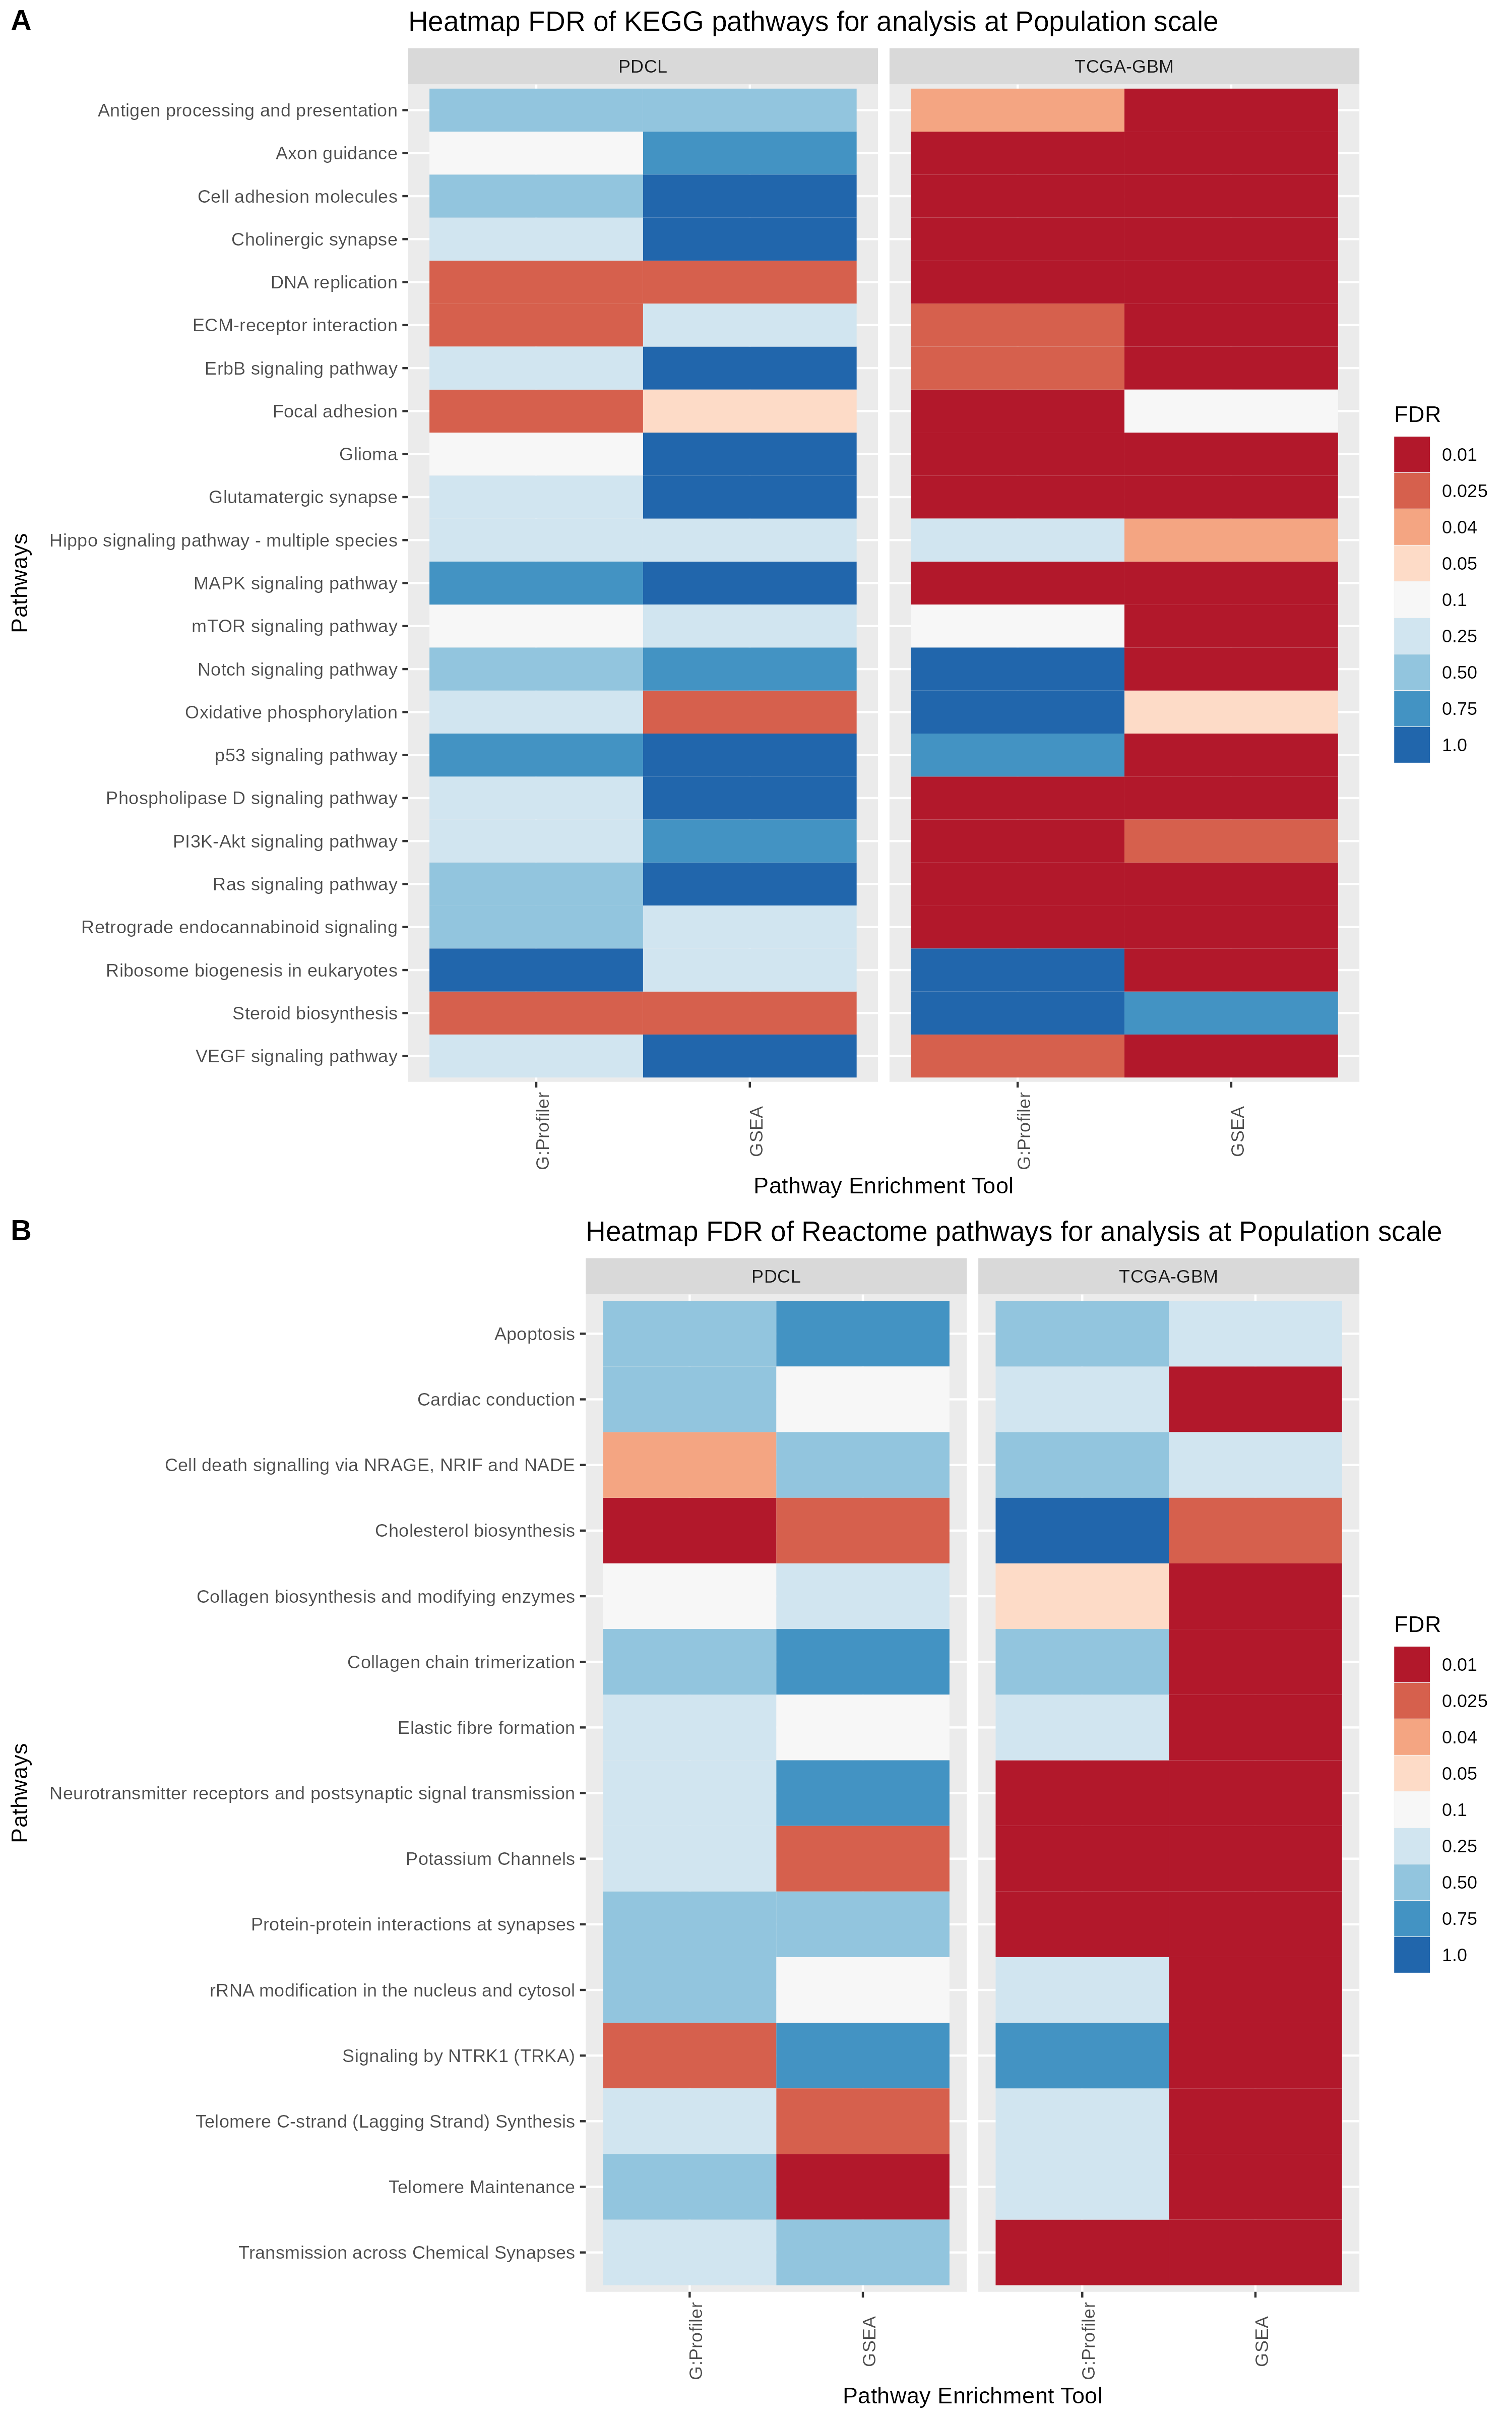
\includegraphics[height=0.7\paperheight]{img/heatmap-fdr-global}
        \caption{
            Heatmap of deregulated pathways in the \acrshort{pdcl} and the \acrshort{tcga} datasets for (A) the \acrshort{kegg} database and (B) the Reactome database.
            \acrshort{fdr} values below 5\% are considered significant (red) and their are not considered significant if greater than 5\% (blue).
        }
        \label{fig:heatmap-fdr-global}
    \end{center}
\end{figure}

The figure \ref*{fig:heatmap-fdr-global}, shows the \acrshort{fdr} values for different pathways from \acrshort{kegg} and Reactome given by G:Profiler and \acrshort{gsea} in both datasets.
As before, we see that a same pathways can be found enriched in one enrichment tool but not in another.
For example, the \acrshort{fdr} for \textit{Oxidative phosphorylation} is significant in both dataset with \acrshort{gsea} but not with G:Profiler.
In \acrshort{tcga}, the \textit{p53 signaling} pathway is found significant only with \acrshort{gsea} and it is not enriched with \acrshort{pdcl} data.
Yet it is found deregulated in one sample during the personnalized analysis of \acrshort{pdcl} samples (described below) suggesting it is rather due to the dataset.
Using pathway enrichment we can also highlights the differences between both datasets.
As an example, many well-known signaling pathways such as \textit{PI3K-Akt signaling}, \textit{RAS signaling} and \textit{VEGF signaling} are found enriched only in \acrshort{tcga}.
At the opposites, pathways involved in cholesterol metabolism such as \textit{Steroid biosynthesis} and \textit{Cholesterol biosynthesis} are found enriched only in \acrshort{pdcl}.
We will show below, that we can assess which samples and the proportions of samples with an altered cholesterol synthesis.

\subsection{Analysis of the deregulated pathways at the individual level}

\subsubsection{Cell adhesion to the ECM is the most frequently deregulated pathway in PDCL samples}

Table \ref*{table:frequently-dereg-pathways-kegg} and \ref*{table:frequently-dereg-pathways-reactome} show the most frequently deregulated pathways in \acrshort{pdcl}.
The \textit{Focal adhesion} (path:hsa04510) is the most frequently deregulated \acrshort{kegg} pathway with 13 samples affected while \textit{Transmission across Chemical Synapses} (R-HSA-112315) is the most frequently deregulated Reactome pathway with 5 samples affected.
Results contain pathways linked to processes influencing the cell motility and its fixation on the matrix such as :\textit{Focal adhesion} (path:hsa04510), \textit{ECM-receptor interaction} (path:hsa04512), \textit{Cell adhesion molecules} (path:hsa04514), \textit{Collagen synthesis} (R-HSA-165814, R-HSA-8948216) and \textit{elastic fibre formation} (R-HSA-1566948).
Glioblastoma cells have the ability to migrate and invade surrounding tissue, sometimes migrating to other organs as well \cite*{Lah2020}, confirming the validity of these results.

In a similar way, \textit{Steroid biosynthesis} and \textit{Cholesterol biosynthesis} are found deregulated in 4 and 3 different samples, respectively.
As we will described more in the Discussion section, cholesterol metabolism has been documented in the litterature to be affected in the case of glioblastoma.

The \textit{Oxidative phosphorylation} (path:hsa00190), well-known for its role in the generation of \acrshort{atp}, is found deregulated in 4 samples.
This pathway has been widely studied due to its important role in the generation of \acrshort{atp} and its potential implication in the Warburg Effect, an increase of usage of glycolysis to produce \acrshort{atp} even though oxygen is available \cite*{Spinicci2022}.
It was first hypothesized that mitochondria were defective in tumour cells, yet it was later mitochondrial function was similar to normal cells \cite*{Cairns2011}.
The \textit{Hippo signaling pathway} (path:hsa04392, path:hsa04390) and \textit{Retrograde endocannnabinoid signaling} (path:hsa04723), two signaling pathway whose role in cancer have been documented in the litterature, are found deregulated in 6 and 5 different samples, respectively.
\todo{read the article about them before citing them as references}

\begin{table}
    \centering
    \resizebox*{\textwidth}{!}{
        \begin{tabular}{ |c|c|c|c|c| }
            \hline
            Database & Pathway ID & Description & Category & Number of PDCL \\
            \hline
            KEGG & path:hsa04510 & Focal adhesion & Cellular Processes & 13 \\
            KEGG & path:hsa04360 & Axon guidance & Organismal Systems & 10 \\
            KEGG & path:hsa04512 & ECM-receptor interaction & Environmental Information Processing & 5 \\
            KEGG & path:hsa04724 & Glutamatergic synapse & Organismal Systems & 5 \\
            KEGG & path:hsa04725 & Cholinergic synapse & Organismal Systems & 5 \\
            KEGG & path:hsa00100 & Steroid biosynthesis & Metabolism & 4 \\
            KEGG & path:hsa00190 & Oxidative phosphorylation & Metabolism & 4 \\
            KEGG & path:hsa04612 & Antigen processing and presentation & Organismal Systems & 4 \\
            KEGG & path:hsa04723 & Retrograde endocannabinoid signaling & Organismal Systems & 4 \\
            KEGG & path:hsa03008 & Ribosome biogenesis in eukaryotes & Genetic Information Processing & 3 \\
            KEGG & path:hsa04012 & ErbB signaling pathway & Environmental Information Processing & 3 \\
            KEGG & path:hsa04072 & Phospholipase D signaling pathway & Environmental Information Processing & 3 \\
            KEGG & path:hsa04392 & Hippo signaling pathway - multiple species & Environmental Information Processing & 3 \\
            KEGG & path:hsa04514 & Cell adhesion molecules & Environmental Information Processing & 3 \\
            KEGG & path:hsa04714 & Thermogenesis & Organismal Systems & 3 \\
            \hline
        \end{tabular}
    }
    \caption{
        Table of the frequently \acrshort{kegg} pathways deregulated in the \acrshort{pdcl}.
        \textit{Focal adhesion} is the most frequently deregulated pathway with 13 samples affected.
    }
    \label{table:frequently-dereg-pathways-kegg}
\end{table}

\begin{table}
    \centering
    \resizebox*{\textwidth}{!}{
        \begin{tabular}{|c|c|c|c|c|}
            \hline
            Database & Pathway ID & Description & Category & Number of PDCL \\
            \hline
            Reactome & R-HSA-112315 & Transmission across Chemical Synapses & Neuronal System & 5 \\
            Reactome & R-HSA-1650814 & Collagen biosynthesis and modifying enzymes & Extracellular matrix organization & 4 \\
            Reactome & R-HSA-5576891 & Cardiac conduction & Muscle contraction & 4 \\
            Reactome & R-HSA-8948216 & Collagen chain trimerization & Extracellular matrix organization & 4 \\
            Reactome & R-HSA-112314 & Neurotransmitter receptors and postsynaptic signal transmission & Neuronal System & 3 \\
            Reactome & R-HSA-191273 & Cholesterol biosynthesis & Metabolism & 3 \\
            Reactome & R-HSA-6790901 & rRNA modification in the nucleus and cytosol & Metabolism of RNA & 3 \\
            Reactome & R-HSA-6794362 & Protein-protein interactions at synapses & Neuronal System & 3 \\
            Reactome & R-HSA-109581 & Apoptosis & Programmed Cell Death & 2 \\
            Reactome & R-HSA-1296071 & Potassium Channels & Neuronal System & 2 \\
            Reactome & R-HSA-1566948 & Elastic fibre formation & Extracellular matrix organization & 2 \\
            Reactome & R-HSA-157579 & Telomere Maintenance & Cell Cycle & 2 \\
            Reactome & R-HSA-174417 & Telomere C-strand (Lagging Strand) Synthesis & Cell Cycle & 2 \\
            Reactome & R-HSA-187037 & Signaling by NTRK1 (TRKA) & Signal Transduction & 2 \\
            Reactome & R-HSA-204998 & Cell death signalling via NRAGE, NRIF and NADE & Signal Transduction & 2 \\
            \hline
        \end{tabular}
    }
    \caption{
        Table of the frequently Reactome pathways deregulated in the \acrshort{pdcl}.
        \textit{Transmission across Chemical Synapses} is the most frequently deregulated pathway with 5 samples affected.
        Collagen pathways are dysregulated in 4 different samples.
    }
    \label{table:frequently-dereg-pathways-reactome}
\end{table}

\begin{figure}
    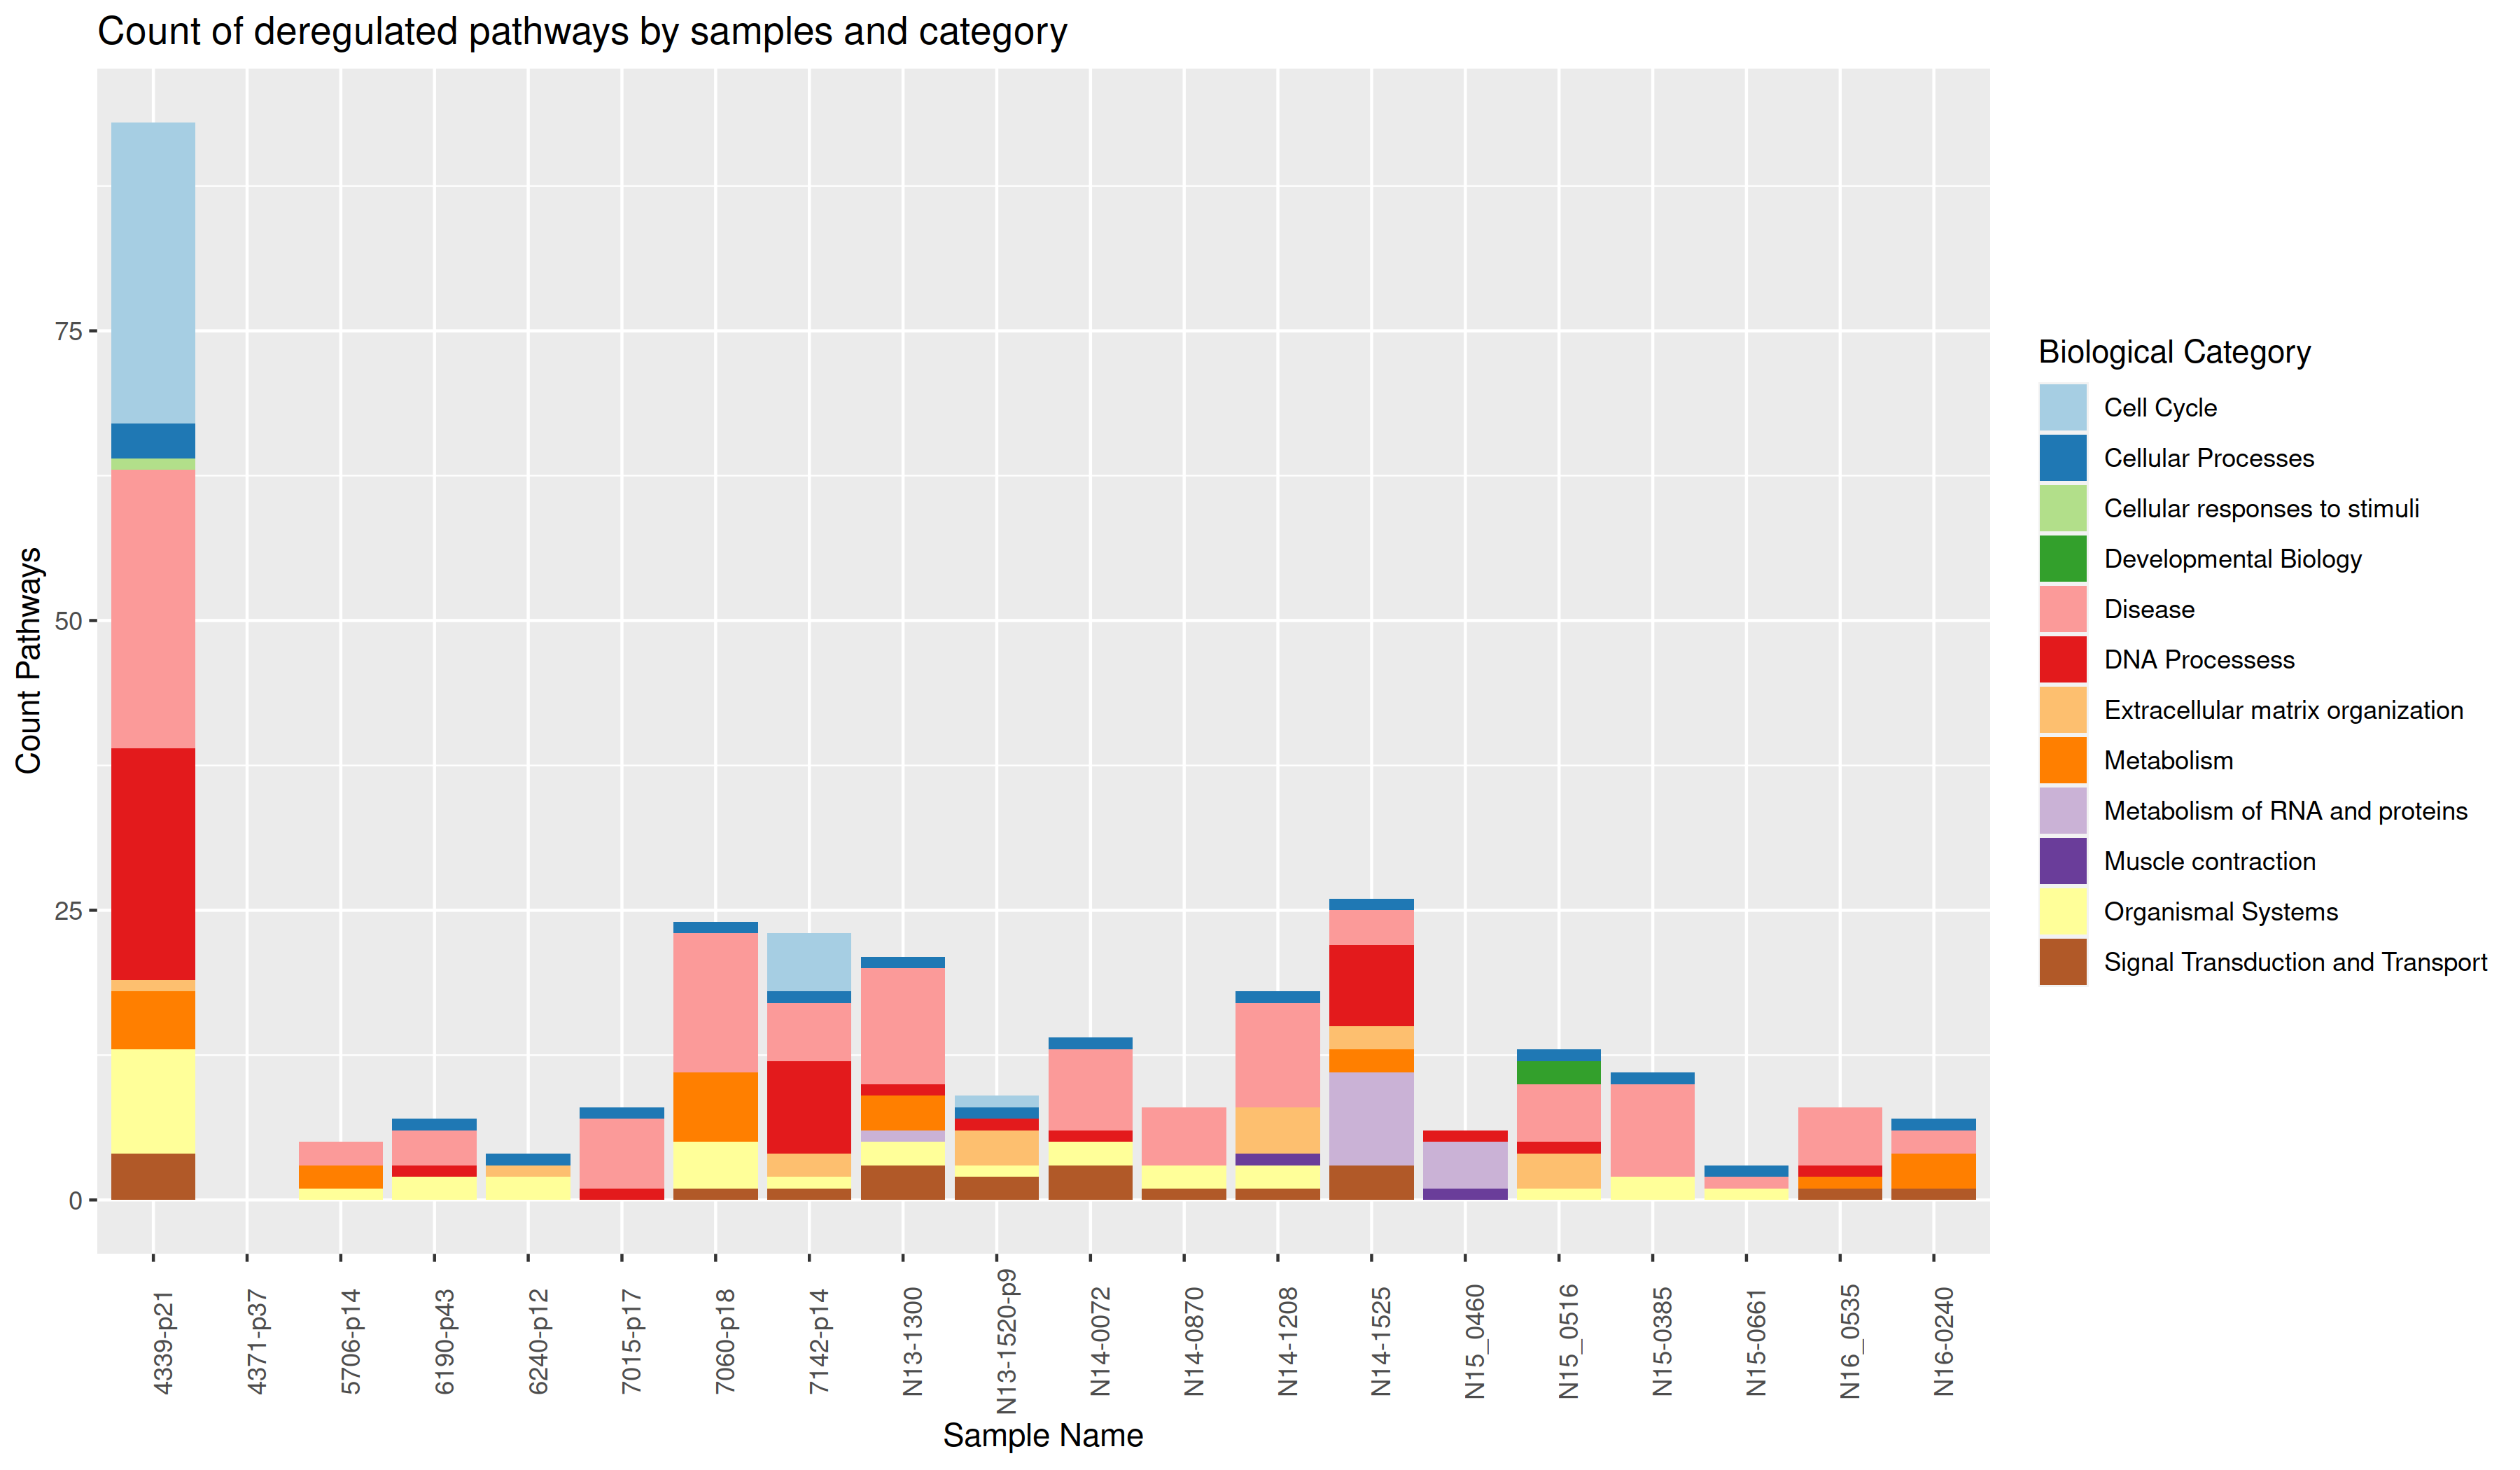
\includegraphics[width=\textwidth]{img/barplot-categ-pdcl}
    \caption{
        Number of deregulated pathways per category and per sample in the \acrshort{pdcl} dataset.
        The  \textit{Human Diseases} and \textit{Organismal Systems} categories are the most frequently deregulated \acrshort{kegg} categories.
        In Reactome, deregulated pathways are often associated with \textit{Neuronal System}, \textit{DNA Repair/Replication} and \textit{Signal Transduction}.
        \textit{4339-p21} is the the sample with the most deregulated pathways in both \acrshort{kegg} and reactome.
        Pathways in this sample are associated to the \textit{Cellular Processes} and \textit{Environmental/Genetic Information Processing} \acrshort{kegg}, or the \textit{Cell-Cycle} Reactome category.
    }
    \label{fig:barplot-categ-pdcl}
\end{figure}

As can be seen in figure \ref*{fig:barplot-categ-pdcl}, the sample \textit{4339-p21} is the most deregulated with around 40 pathways significantly enriched in both \acrshort{kegg} and Reactome.
Most of the pathway found deregulated with the \acrshort{kegg} database, across all the \acrshort{pdcl} samples, are associated to \textit{Human Diseases}.
\textit{Human Diseases} aside, the majority of deregulated pathways in the sample \textit{4339-p21} are associated to the \textit{Cellular Processes} and \textit{Environmental/Genetic Information Processing} \acrshort{kegg}, or the \textit{Cell-Cycle} Reactome category.

\subsubsection{Sample clustering by their deregulated categories}

\begin{figure}
    \begin{center}
        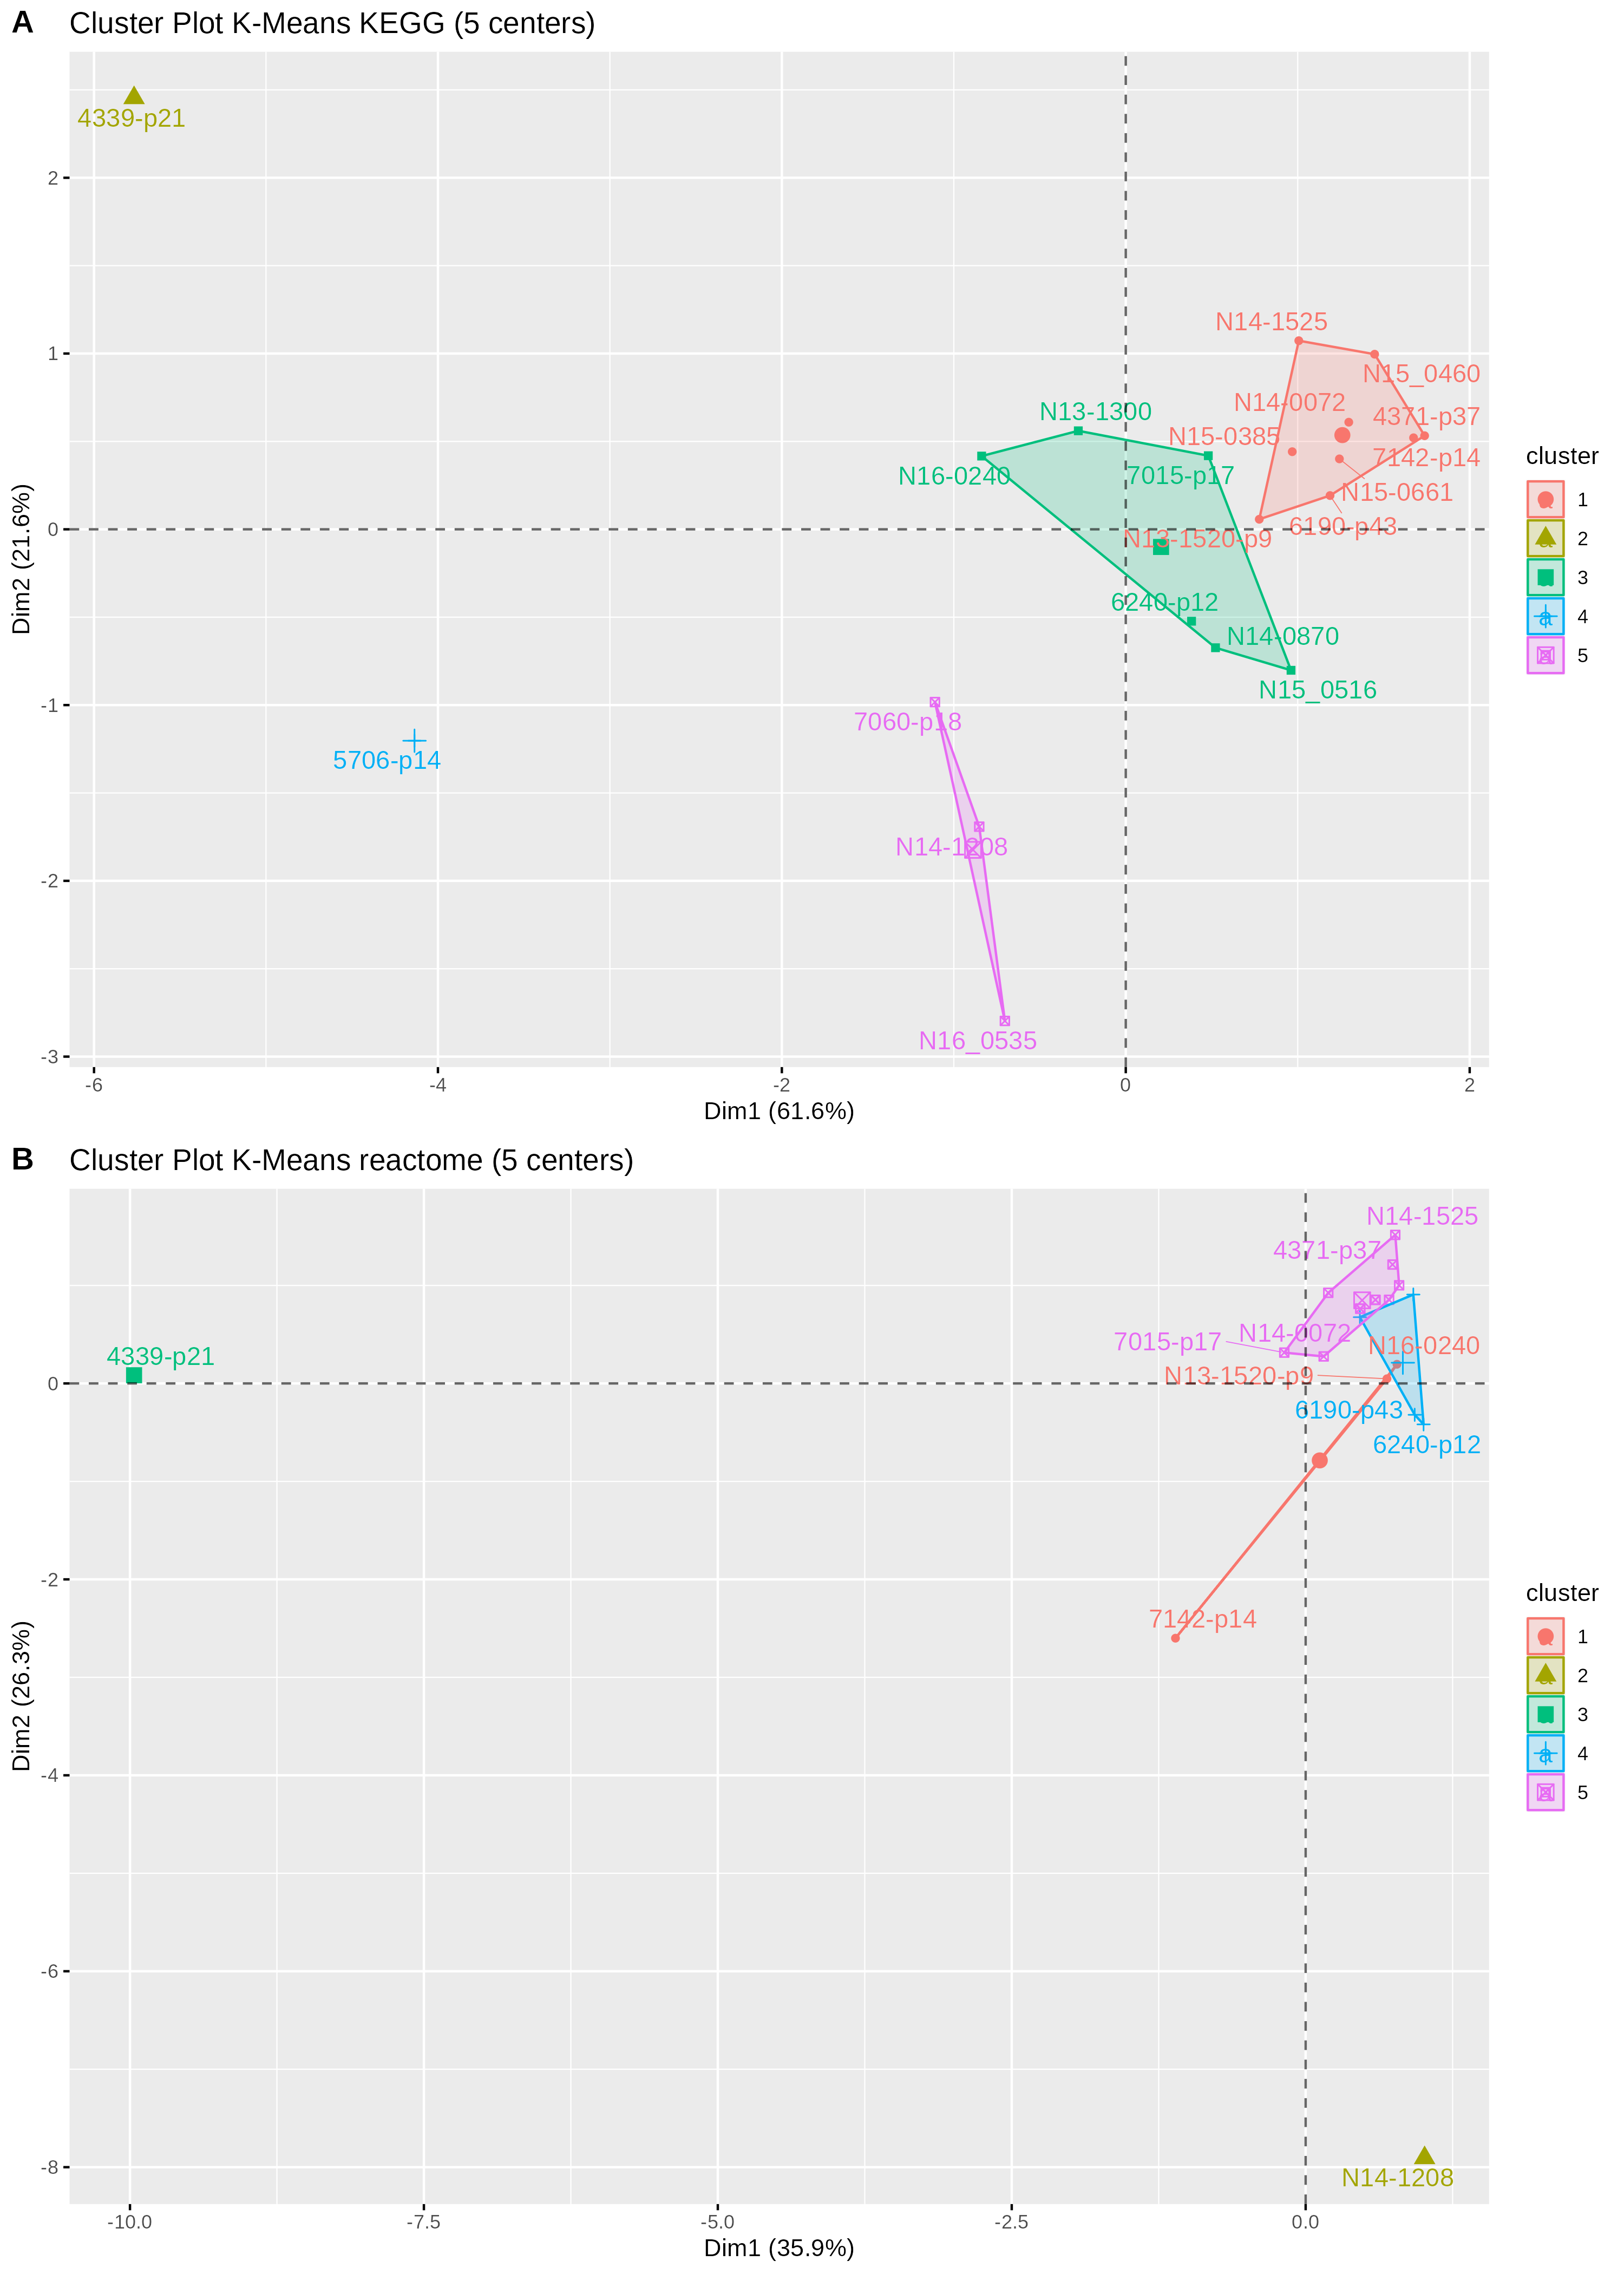
\includegraphics[height=0.6\paperheight]{img/plot_cluster_pdcl}
        \caption{
            Clustering of the \acrshort{pdcl} samples using the percentage of deregulation per biological categories.
            Results are shown with (A) \acrshort{kegg} categories and (B) Reactome categories.
            To generate a vector of values for each samples, we divided the number of pathways found significantly enriched for a category by the number of total pathways in this category present in the \acrshort{gmt} file.
            Clustering was done using the K-Means method with 5 clusters.
        }
        \label{fig:cluster-plot-pdcl}
    \end{center}
\end{figure}

For each samples, we divided the number of pathways deregulated in a category by the total number of pathways associated to this category in the \acrshort{gmt} file.
We used the vector of values generated to perform clustering of the samples using the K-Means algorithm with 5 clusters.
Results are shown in figure \ref*{fig:cluster-plot-pdcl} for \acrshort{kegg} and Reactome categories.
There is a better delimitation of the cluster using \acrshort{kegg} categories than with Reactome where three clusters overlap a little.
Although the sample \textit{4339-p21} is separated from others samples in both \acrshort{kegg} and Reactome, the clusters deined depend on the database.
This shows how analyses of pathway enrichment results can vary depending on the database used.
Reactome has more categories defined and used for clustering than \acrshort{kegg} (6 for \acrshort{kegg} and 16 for Reactome).
Thus, filtering the \acrshort{gmt} file to include fewer categories may improve the result when performing clustering.
With \acrshort{kegg} clustering, the first dimension separate samples based on the total number of deregulated processes.
The second dimension separate samples with deregulated pathways associated with the \textit{ Metabolism }, \textit{ Cellular Processes} and \textit{Genetic Information Processing} from the samples with deregulated pathways mainly associated with the \textit{ Organismal Systems }, \textit{Environmental Information processing} and \textit{Human Diseases} categories.
With Reactome clustering, the first dimension seems to separate samples with deregulated processes associated with the Cell-Cycle, DNA replication/repair, Gene expression, Signal Transduction and Immune System.
The second dimension separate samples with processess of the Metabolism deregulated from samples with processes linked to the \acrshort{ecm}, Neuronal System, Disease, Transport of small molecules and others.